\section{Bib{\TeX} tools}

http://tex.stackexchange.com/questions/174509/is-there-a-tool-service-that-can-enrich-a-bibtex-database

https://github.com/joosbuijs/bibcleaner

\subsection{JabRef}
JabRef is an open source project, currently developed and maintained
by Jörg Lenhard, Matthias Geiger, Oliver Kopp, Simon Harrer and Stefan
Kolb\cite{jabref_developers}.  It is using the pure Bib{\TeX} format
and has features for automatic key generation, searching online
databases and a plugin system\cite{jabref_features}.  There is a
feature for handling Journal Abbreviation using predefined lists of
abbreviations\cite{jabref_abbreviations}.  Currently JabRef does not
have any spell checking features, but is planned for the next full
release\cite{jabref_spellchecker}.

The JabRef team is currently working on a tool named CloudRef which
has a focus on a web based interface for collaboration.  Currently the
project is in the planning phase and suggested features hints that it
might end up correcting some of the issues, as there is some focus on
correctly filled Bib{\TeX} references and corrections for those.

Looking through the lists of JabRef plugins does not reveal any that provide
solutions to the given issues.  There are a lot of plugins for lookups
in online databases, which can offer a partial solution (provided the
online information is correct and that it is there for the reference)
for new entries\cite{jabref_resources}.  Since JabRef uses Bib{\TeX}
for storage, tools for Bib{\TeX} can be used too.

When using JabRef it is very easy to switch between journal
abbreviations and full names, provided that the abbreviation is
already known, custom abbreviations can be
added\cite{jabref_abbreviations}.  The supposed spell check was not to
be found in the beta release of JabRef.  Doing lookups online for
details can in theory be done during PDF-import using Mr. DLib, which
supposedly should search for entries based on similarity to PDF-files,
the project seems to be abandoned as the site has not been updated
since 2012\cite{jabref_mrdlib,jabref_mrdlib_notice}.  It is worth
nothing that JabRef has a system for finding duplicate entries, and
does some validation of Bib{\TeX}-files when opened to ensure valid
data.

\section{Other bibliography tools}
There are a lot of different bibliography management software.  Some
of these provides partial solutions for the lexical and consistency
concerns.  All of the tools have been tested for relevant features
that are not described on their respective feature overviews.

\subsection{Mendeley}
Mendeley is a bibliography management tool developed by Mendeley Ltd.
The focus of the tool is to make it easy to manage and share
references.  Mendeley provides features such as importing PDF-files
and detecting relevant details such as the author, title and DOIs, and
updating entries from online databases using, for instance the DOI.
The target group for Mendeley is students and researchers
\cite{mendeley_features}.

Like BibTeX, Mendeley does not facilitate any systems for detecting
inconsistencies such as spelling errors, revision numbers or initials.
Mendeley can download metainformations based on a DOI which in part
remodies this.  Mendeley does not have any plugin/add on system, so
it's unlikely that there is any third party tools to remedy this. A
search through Mendeley's request database reveals the same as the
testing and features page.  On Mendeleys online request system there
are requests for features such as: spell checking, fixing
capitalization inconsistencies and bulk DOI lookups.
\cite{mendeley_request_spellcheck, mendeley_request_lowercase,
  mendeley_request_capitalization, mendeley_request_bulk_doi}.

\subsection{EndNote and RefMan}
EndNote and RefMan also tools for reference mangement, made by
Thompson Reuters.  RefMan is an older product and Thompson Reuters
recommends using EndNote in stead \cite{refman_switch,
  refman_features}.  There is a lot of focus on the sharing
capabilities and provides tools for PDF import and management, online
lookup of references and Journal abbreviation dection
\cite{endnote_basic_features, endnote_x7_features}.  Their target
group is students and university related groups.  EndNote also
provides a spell check feature that is not mentioned in the feature
sets\cite{endnote_spellcheck}.

The tools for handling abbreviations in EndNote is only used to format
the names when exported or used as references.  This is done using a
mapping from a predefined set of know abbreviations, the tool does not
fix the naming issues internally in the
files\cite{endnote_terms_journals}.

When trying to remedy the spelling and consistency errors by using DOI
lookups it seems that the only way of doing that will create duplicate
entries rather than updating the current one. This is just making the
issues even worse as the references then ends up with duplications
too.  The spell checker works on a per entry basis and there is no
apparent way to spell check an entire bibliography.  EndNote provides
a lot of extra downloads to provide features such as Bib{\TeX}
support, however no downloads were found to remedy neither the lexical
nor the consistency concerns further\cite{endnote_downloads}.

\subsection{RefWorks}
RefWorks is a web based reference manager developed by ProQuest, meant
for students, researchers and librarians.  The focus of the tool is to
have the simplicity of a web based solution, which makes the resources
easy to share and available everywhere.  The features include online
look ups, statistics systems and collaboration
features\cite{refworks_features}.

As with the other tools testing shows that the error detection
features is limited.  In RefWorks the work flow for adding references
is to either enter them manually or to use a browser link called
``RefGrab-It'' to import from homepages.  As with the DOI lookups
(which it can import if you look up a DOI resource in your browser)
this in part remedy the errors, provided the original source does not
have them.  Contrary to the other tools RefWorks tries to detect if
the author name is malformed, although it only seems to detect if you
type ``John Doe'' rather than ``Doe, John'' as it expects, as can be
seen at figure-\ref{fig:refworks-detect-formatting}.

\begin{figure}[h]
    \centering
    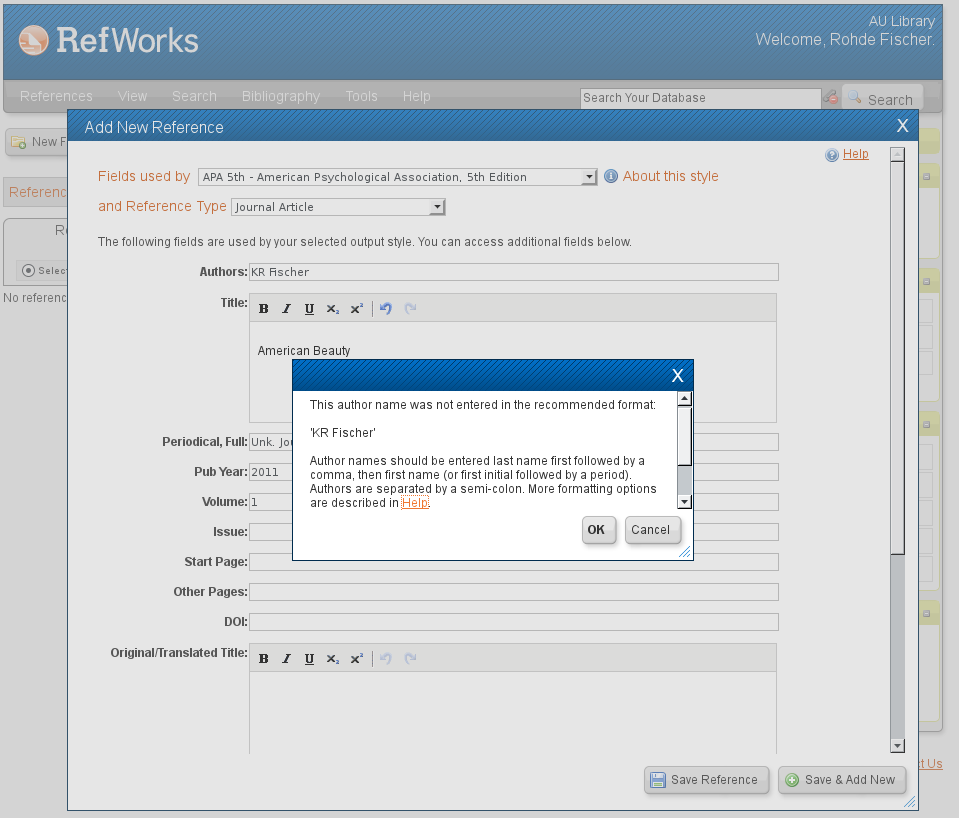
\includegraphics[width=0.8\textwidth]{refworks-detect-formatting}
    \caption{RefWorks detects some formatting on the name field}
    \label{fig:refworks-detect-formatting}
\end{figure}

In RefWorks itself there seems to be no spell checker, but this is in
part solved by most modern browsers, because they tend to include
spell checkers for input fields.

\subsection{Zotero}
Zotero has a built in spell checker for notes, however the spell
checker is not applied for things like titles, which prevents it from
detecting those errors.  Also it does not seem that it does anything
to detect abbreviations.  Unfortunately Zotero does not have a list of
features directly, apart from some very superficial texts on the front
page \cite{zotero_features}.

Unlike the other systems Zotero has a plugin system, which makes it
possible that a user created plugin for these features exists, however
none was found using the official list of plugins
\cite{zotero_plugins} nor by a normal search engine.

There is a limited mechanism for detecting abbreviations in Zotero, in
its jar-file there is a list of known abbreviations which it can use
to chose the correct abbreviation when exporting, entering a known
abbreviation does not seem to correct it to the non-abbreviated
version.  This list can be manually edited, and overruled
\cite{zotero_abbreviations}

%%% Local Variables:
%%% mode: latex
%%% TeX-master: "thesis"
%%% End:
